% REMEMBER: You must not plagiarise anything in your report. Be extremely careful.

\documentclass{l4proj}

    
%
% put any additional packages here
%

\begin{document}

%==============================================================================
%% METADATA
\title{Level 4 Project Report Template}
\author{John H. Williamson}
\date{September 14, 2018}

\maketitle

%==============================================================================
%% ABSTRACT
\begin{abstract}
    Every abstract follows a similar pattern. Motivate; set aims; describe work; explain results.
    \vskip 0.5em
    ``XYZ is bad. This project investigated ABC to determine if it was better. 
    ABC used XXX and YYY to implement ZZZ. This is particularly interesting as XXX and YYY have
    never been used together. It was found that  
    ABC was 20\% better than XYZ, though it caused rabies in half of subjects.''
    \begin{itemize}
        \item what is LBD?
        \item what will this project do?
        \item what is the result of this project?
    \end{itemize}
\end{abstract}

%==============================================================================

% EDUCATION REUSE CONSENT FORM
% If you consent to your project being shown to future students for educational purposes
% then insert your name and the date below to  sign the education use form that appears in the front of the document. 
% You must explicitly give consent if you wish to do so.
% If you sign, your project may be included in the Hall of Fame if it scores particularly highly.
%
% Please note that you are under no obligation to sign 
% this declaration, but doing so would help future students.
%
\def\consentname {Timothy Baldock} % your full name
\def\consentdate {30 January 2024} % the date you agree
%
\educationalconsent


%==============================================================================
\tableofcontents

%==============================================================================
%% Notes on formatting
%==============================================================================
% The first page, abstract and table of contents are numbered using Roman numerals and are not
% included in the page count. 
%
% From now on pages are numbered
% using Arabic numerals. Therefore, immediately after the first call to \chapter we need the call
% \pagenumbering{arabic} and this should be called once only in the document. 
%
% Do not alter the bibliography style.
%
% The first Chapter should then be on page 1. You are allowed 40 pages for a 40 credit project and 30 pages for a 
% 20 credit report. This includes everything numbered in Arabic numerals (excluding front matter) up
% to but excluding the appendices and bibliography.
%
% You must not alter text size (it is currently 10pt) or alter margins or spacing.
%
%
%==================================================================================================================================
%
% IMPORTANT
% The chapter headings here are **suggestions**. You don't have to follow this model if
% it doesn't fit your project. Every project should have an introduction and conclusion,
% however. 
%
%==================================================================================================================================
\chapter{Introduction}

% reset page numbering. Don't remove this!
\pagenumbering{arabic} 

\section{Motivation}
\begin{itemize}
    \item Scale of research
    \item Cost of machine learning
\end{itemize}

\section{Aims}
\begin{itemize}
    \item Explore different aspects of MeSH tags in lbd
    \item Give pointers on what variations are useful
\end{itemize}

\section{Dissertation Outline}
\begin{itemize}
    \item Background
    \item Analysis
    \item Implementation
    \item Evaluation
    \item Conclusion
\end{itemize}

%==================================================================================================================================
\chapter{Background}

\section{Increase in Research Rate}

The global research rate is increasing. This is in part fueled by the global spending on research and development has increased to 2.4 trillion dollars in 2020 from only 675 billion in 2000 as reported by the Congressional Research Service (2022). As research across the world continues to grow, so to does our accumulated knowledge grow. According to Bornmann and Lutz (2015) \textbf{ref}, the rate of research increased exponentially between 1980 and 2013, with a growth rate of about 3\% for global scientific publications in this time frame. With an ever growing repository of information it becomes more difficult to accumulate expertise in a field. This is further exacerbated by the increasing rate of research which also makes it trickier for individual experts to stay up to date with developments in their field. \\ 

The result of this, is a narrowing of expertise as discussed by Swanson et al. \textbf{ref}. To become expert in a field requires increasingly more time to be spent on a narrower area of a field. A consequence of this is that individuals can benefit less from their wider understanding of their field as not only can they spend less time learning about the broader subject but also the required time taken to properly develop knowledge in other parts of their field increases.\\ 

\section{Introduction of Literature Based Discovery}

Here is where literature based discovery, LBD, comes in. LBD is the idea that we can use this vast and ever growing database to generate hypothesis for future work. Henry and McInnes \textbf{ref} provide many examples of LBD's applications and achievements including identifying potential treatments for cancer and finding treatments for cataracts. Biomedical research is the field in which LBD is most utilised, but there are numerous instances of its use in other fields. Aamot's work with using it for oceanographic climate science is a case of LBD being applied to another field with its application in studying climate change. Given the increasing quantity and funding of research, being able to effectively generate hypothesis by linking different areas expertise will only become more crucial.\\  

\section{PubMed}

PubMed is a system to help with the organising and searching of life science and biomedical literature. It was created by the National Center for Biotechnology Information and contains the abstract and other key information of over 36 million publications. The primary feature of PubMed is MEDLINE, a system containing citations from selected journals and articles indexed by MeSH tags. \\

\subsection{MeSH Tags}
\begin{itemize}
    \item Introduction
    \item Creation and Structure
    \item Role of MeSH in information retrieval 
    \item benefits as data 
    \item Expert summary
    \item Key information of a paper
    \item easier to process
    \item problems as data
    \item limited information compared to full text
    \item Evolving medical terminology
\end{itemize}

MeSH tags are a system of labels used to identify and categorise biomedical articles in the PubMed database. MeSH tags provide a standardized set of terms to describe the subject matter of articles. This ensures consistency in indexing and searching across different databases and publications and is controlled by the National Library of Medicine. They were made publically available in 1996 and have been key to searching and organising biomedical literature since. By keeping the scope of terms controlled, the National Library of Medicine can ensure that similar concepts are labelled in a consistent manner, irrespective of different cultures and languages across the world. This is very important in a globally researched subject The MeSH database is regularly updated and expanded to reflect advances in biomedical research and changes in terminology. New terms are added, and existing terms are revised to ensure accuracy and relevance in a continuously evolving field. 

\begin{figure}[h]
    \centering
    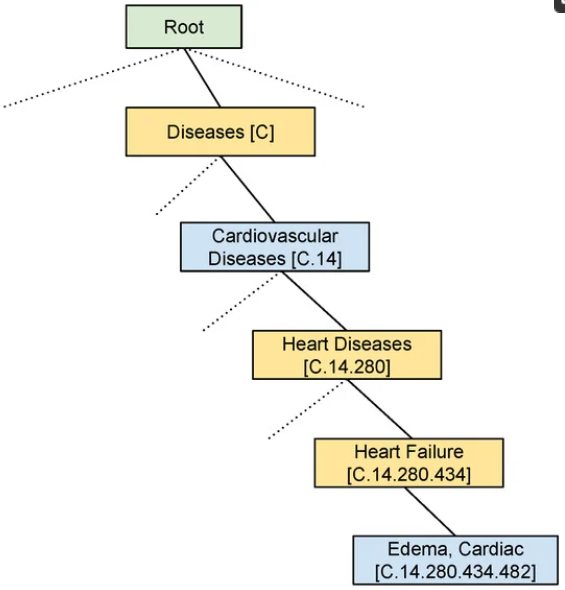
\includegraphics[width=0.6\linewidth]{images/mesh_label.png}
    \caption{image from: Integrating PubMed Label Hierarchy Knowledge into a Complex Hierarchical Deep Neural Network}
    \label{fig:mesh}
\end{figure}
 

\section{Swanson's ABC System}

\begin{figure}
    \centering
    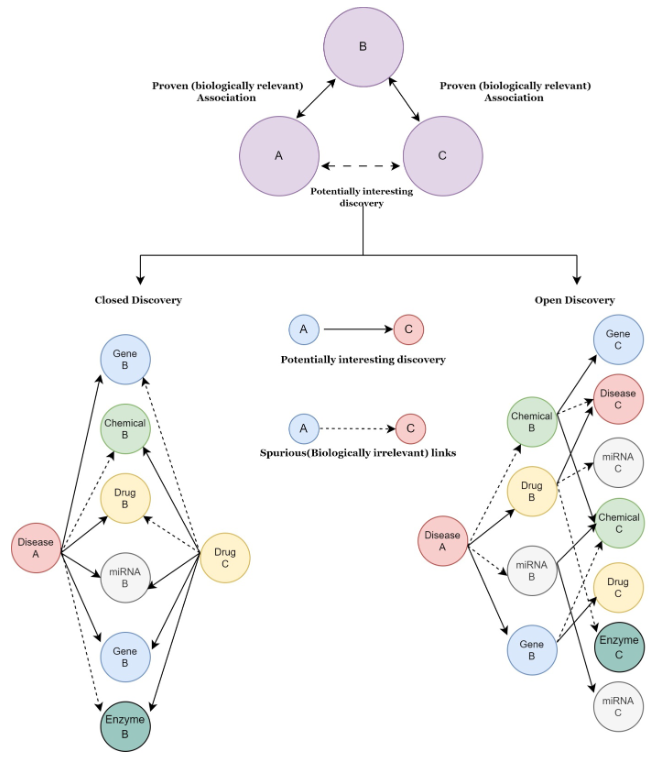
\includegraphics[width=\linewidth]{images/abc_open_closed.png}
    \caption{image from: Literature Based Discovery (LBD): Towards Hypothesis Generation and Knowledge Discovery in Biomedical Text Mining}
    \label{fig:open_closed}
\end{figure}

LBD is founded on Swanson's ABC approach. In this approach, if concepts A and B have an established relationship, and concepts B and C do too, then there may well be a transitive relationship between A and C. This is visualised at the top of Figure \ref{fig:open_closed} where A and B, and B and C are linked by proven association and so the link between A and C might be a potentially interesting discovery. In particular, this system is interested in circumstances where no relationship between A and C has been previously established as this might therefore be a new connection that could be discovered. An example of this being successfully implemented by Swanson himself would be his discovery of using fish oil to treat Raynard's disease. \\

Open and closed discovery are the two main methods of Swanson's ABC system. Open discovery involves the user to have an identified concept A for which to discover possible C concepts. This can be done by identifying all the possible C concepts that are not linked to the original A but have at least one B concept in common with A. The connection between A and each C can then be evaluated by some metric and used to sort the possible C concepts in some way so that they can be returned to the user in meaningful manner. In this way, Open discovery can be used to answer the questions of what concepts are connected indirectly to a given concept and how they might compare to each other. \\

Closed discovery, on the other hand, seeks to answer entirely different questions. This system requires pre-given A and C concepts so that the B connections between them can be discovered. This allows the user to check if any common ground can be found between two concepts that they might suspect have a connection. This could even be generalised beyond unconnected concepts, it could be used to explore new ways two concepts, that have pre-existing connections, might be overlapping. Closed discovery therefore asks the question of how or why two concepts are connected. The two concepts do not have to exist in isolation of each other. In fact, since they answer very different questions they can be used in combination with each other to first discover new connections and then to explore why those concepts are connected. In this way Swanson created an effective and comprehensive approach to LBD, laying the groundwork for the development that followed. \\ 

\section{Discovery Methods}

\begin{figure}[h]
    \centering
    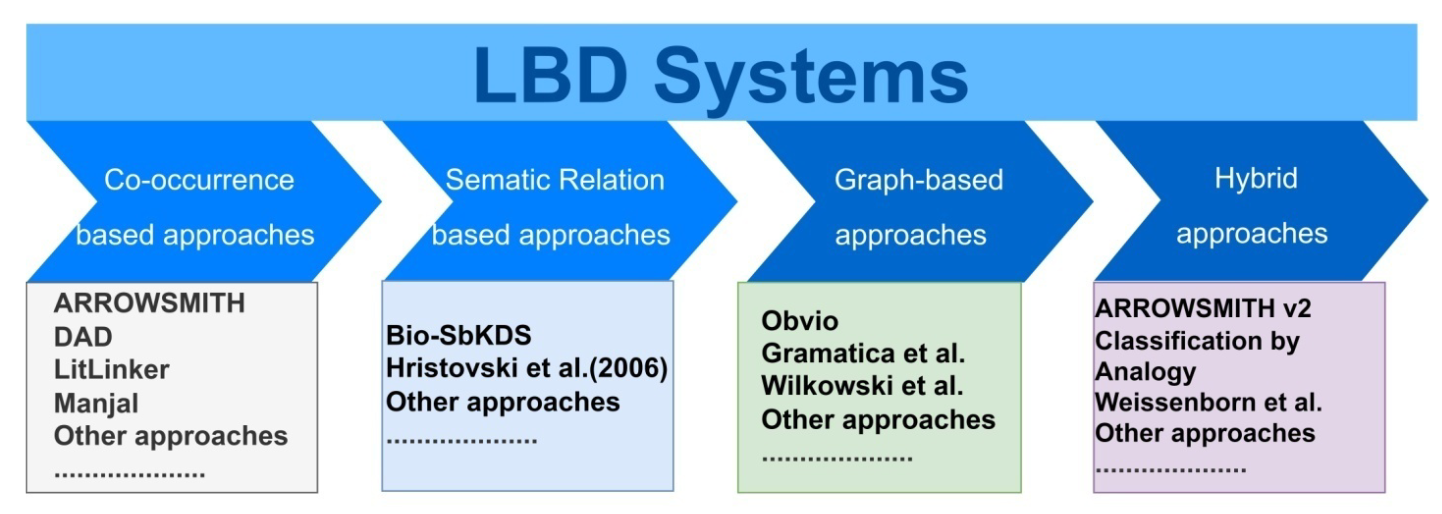
\includegraphics[width=\linewidth]{images/lbd_discovery_methods.png}
    \caption{image from: Literature Based Discovery (LBD): Towards Hypothesis Generation and Knowledge Discovery in Biomedical Text Mining}
    \label{fig:discovery_methods}
\end{figure}

Ultimately LBD depends on the proficiency of its discovery methods. Furthermore, for LBD to grow in use and to keep up with developing data analysis techniques, it must continue to improve the systems of discovery. Figure \ref{fig:discovery_methods} displays a rough outline of the progression of LBD systems and provides some umbrella concepts that allow the grouping of similar designs. There are have been several different approaches over the years which are worth exploring further. \\

\subsection{Co-occurence Approaches}

Using this ABC system, Swanson went on to developed the Arrowsmith search system. This is a co-occurence based system, where links between concepts are determined by if they both occure in the same paper's title. The objective of this tool is to make the ABC system more accessible and usable for researchers to actually use without having to build their own version of the system from scratch. The system implements the closed discovery system, allowing researchers to explore links between two pre-chosen concepts that they are looking to explore. \\

It functions by searching article titles in Medline, a biomedical database of citations and abstracts. It searches these titles for terms A and C, and returns a file for each respective term containing all of the titles with that term. The next step is for the Arrowsmith software to compare the two files and create a list of all 'B' terms that appear on both files. From here a stop word list of the 5000 most common terms is used to filter out the obviously redundant words from the list. \\

At this stage, the user can then filter the list further by taking out terms that they know are not relevant or interesting. Furthermore, the list can be automatically filtered further to only give terms that appear at least twice in both of the A and C files. This gives the user an easier way to significantly reduce the returned terms if they are dealing with a particularly long list. Using this finalised list, the system will return a list of titles containing both the A and B terms, and the B and C terms. From this, the user will be able to determine if they think there are any links between these concepts worth exploring. \\

In this way, Arrowsmith can be a useful tool for exploring connections between concepts. This is irrespective of whether or not there is a pre-existing connection between concepts A and C. It could for example be used to discover new links between two concepts that we already know are connected but want to explore further. However, a draw back of this system is that it is heavily reliant on the user being an expert in the field and having a wealth of experience at reading and understanding biomedical publications. \\ 

\subsection{Semantic Relation Approaches}

Another approach to LBD is utilising semantic relations to create more confident and accurate predictions. Hu et al. developed a system called Bio-sbKDS, Biomedical Semantic-based Knowledge Discovery System, that uses biomedical ontologies to try to fully automate the process of refining predictions. The benefit of this is it should greatly reduce the time and effort an expert would have to input to produce a meaningful result. By using semantic networks such as UMLS, Unified Medical Language System, the system can better identify connections that are worth investigating. In this way, this system implements Swanson's open discovery system, allowing users to discover concepts linked by specific relationships. To make these predictions, Bio-sbKDS takes in the following information from the user. 
\\ 
\begin{itemize}
    \item \textbf{Starting concept}, a keyword to represent the concept that the user wants to discover concepts that link to it. \\
    \item \textbf{Semantic relationship}, the desired relationship that the user is interested in between the given concept and the discovered concepts. \\
    \item \textbf{Date range}, a set of dates to limit the searched publications to. \\
\end{itemize}

Using these inputs, the user is able to significantly focus the output of the system towards what they are looking for. Furthermore, by reducing the date range to a relevant window for their particular research, the user can significantly cut down on the time taken for the system to process the data. \\

\subsection{Graph-based Approaches}

One aspect of graph based approaches is the idea of formatting and storing the information as a graph. This would be instead of the standard relational tables used for SQL, structured query language, as these tables don't make as much sense for data that is in the form of a network as opposed to distinct objects. Instead, if this can data can be formatted in storage as a graph, it could be more straightforward and more effective for accessing in LBD. \\

With this in mind, Hristovski et al. used Neo4j to graph database for LBD. Neo4j is a noSQL, commonly thought of as not only SQL, technology that allows the creation of a database that stores data in the form of a graph comprised of nodes and edges. Neo4j therefore has its own query language, Cypher, for accessing its data. With this query language, both open and closed discovery can be implemented on the database, allowing the previously described systems to be re-implemented using this technology. Cypher has the functionality to satisfy these systems, as it can both run simple commands that only care about co-occurrence, or more complicated ones that filter by concept and semantic relationship type. \\

However, implementation of this system did face some problems. When using the LOAD CSV command, for loading text data into the system, it failed to load all of the data, only managing the first few million instances. In addition, if the user wishes to place further stipulations on the nature of the concepts and relationships they want returned, the authors found that the queries would take longer to process. When the researchers built this system in 2015, Neo4j was version 2.1.6 and had two types of indexing, legacy indexes and schema indexes. The legacy indexes are not recommended as they are difficult to use, but they provide the desired text, node, and relational indexing. The ability to fully index text and relations is not provided by the recommended schema index. \\

\section{Machine Learning}
\begin{itemize}
    \item history/introduction
    \item Text representation
    \item Deep learning
    \item Domain specific challenges
    \item Ethical considerations
\end{itemize}

\section{PubMed}
\begin{itemize}
    \item Ethical concerns of LBD
    \item Copyright
    \item Data Privacy
    \item what is it
    \item why use it
\end{itemize}

\section{MeSH Tags}
\begin{itemize}
    \item Introduction
    \item Creation and Structure
    \item Role of MeSH in information retrieval 
    \item benefits as data 
    \item Expert summary
    \item Key information of a paper
    \item easier to process
    \item problems as data
    \item limited information compared to full text
    \item Evolving medical terminology
\end{itemize}

%==================================================================================================================================
\chapter{Analysis}
\section{Document and Term Representation}
\begin{itemize}
    \item How to represent a document
    \item How to represent a term
    \item How to represent a Relationship
\end{itemize}
\section{Data Processing}
\begin{itemize}
    \item What data do we want
    \item How do we want to represent it
\end{itemize}
\section{Swanson ABC}
\begin{itemize}
    \item point
\end{itemize}
\section{Machine Learning}
\begin{itemize}
    \item time/resource cost
    \item future in data analysis
    \item link prediction vs classifiers
    \item Recommender systems
\end{itemize}
\section{MeSH Tags}
\begin{itemize}
    \item Biomedical Text mining using MeSH
    \item benefits as data 
    \item Expert summary
    \item Key information of a paper
    \item easier to process
\end{itemize}

%==================================================================================================================================
\chapter{Implementation}
\section{Data Processing}
\begin{itemize}
    \item Filtering the data
    \item Transforming into dictionaries
    \item Pickling the constructs
\end{itemize}
\section{Knowledge Graphs}
\begin{itemize}
    \item Networkx
    \item Creating small ones to ensure correct
    \item Common functions to create graphs
\end{itemize}
\section{Swanson ABC}
\begin{itemize}
    \item Used the small graphs to test my implementation
    \item Common functions
    \item Evaluating with hits@k
\end{itemize}
\section{Machine Learning}
\begin{itemize}
    \item pytorch
    \item using tutorial
    \item Converting to homogeneous
    \item Data problems
    \item bug fixing problems
    \item Implementing evaluation
\end{itemize}

\chapter{Evaluation} 

\chapter{Conclusion}    

\begin{appendices}

\chapter{Appendices}

Typical inclusions in the appendices are:

\begin{itemize}
\item
  Copies of ethics approvals (required if obtained)
\item
  Copies of questionnaires etc. used to gather data from subjects.
\item
  Extensive tables or figures that are too bulky to fit in the main body of
  the report, particularly ones that are repetitive and summarised in the body.

\item Outline of the source code (e.g. directory structure), or other architecture documentation like class diagrams.

\item User manuals, and any guides to starting/running the software.

\end{itemize}

\textbf{Don't include your source code in the appendices}. It will be
submitted separately.

\end{appendices}

%==================================================================================================================================
%   BIBLIOGRAPHY   

% The bibliography style is abbrvnat
% The bibliography always appears last, after the appendices.

\bibliographystyle{abbrvnat}

\bibliography{l4proj}

\end{document}
